\documentclass[11pt]{article}
\usepackage[margin=0.92in]{geometry}
\usepackage{amsmath,amssymb,amsthm,mathtools}
\usepackage[T1]{fontenc}
\usepackage{lmodern}
\usepackage{graphicx}
\usepackage{float}
\usepackage{xcolor}
\usepackage[hidelinks]{hyperref}

\newtheorem{theorem}{Theorem}
\newtheorem{lemma}[theorem]{Lemma}
\newtheorem{corollary}[theorem]{Corollary}
\newtheorem{remark}[theorem]{Remark}
\newcommand{\N}{\mathbb N}
\newcommand{\Z}{\mathbb Z}
\newcommand{\ud}{\underline d}

\title{Positive-Density Two-Sided Product Escape for\
Frequently Hypercyclic Bilateral Shifts}
\author{Candidate partial result for arXiv:1305.2325}
\date{13 August 2026}

\begin{document}
\maketitle

\begin{center}
\fcolorbox{black}{gray!8}{\parbox{0.88\linewidth}{
\textbf{Status: candidate partial result, pending human review.}
For every invertible frequently hypercyclic bilateral weighted shift on
$c_0(\Z)$, both one-sided cumulative products escape in the required
directions along one set of positive lower density.  A tail-richness condition
on the standard witness family then implies that the inverse is frequently
hypercyclic.  The unrestricted bilateral-shift inverse problem remains open.}}
\end{center}

\section{The surviving problem}

Let $w=(w_n)_{n\in\Z}$ be a bounded and bounded-below sequence of positive
weights and let $B_w e_n=w_ne_{n-1}$ on $c_0(\Z)$.  Put
\[
 W_r=\prod_{\nu=1}^r w_\nu,
 \qquad L_r=\prod_{\nu=-r+1}^{0}w_\nu
 \qquad(r\geq1).                                                       \tag{1}
\]
Bayart and Ruzsa ask whether frequent hypercyclicity of an invertible
$B_w$ forces frequent hypercyclicity of $B_w^{-1}$ \cite{BR}.  Their PDF
contains the evident typo ``is $T^{-1}$ invertible?''; the next paragraph and
their partial theorem make the intended question unambiguous.

\begin{figure}[H]
  \centering
  
\includegraphics[width=\textwidth]{figures/source_question.png}
  \caption{The question and bilateral-shift specialization in
  arXiv:1305.2325, PDF page 16.}
\end{figure}

Menet later answered the question negatively for general operators on
$\ell^1$ \cite{Menet}.  The special bilateral-shift problem, however, is
explicitly retained in Grosse-Erdmann's later characterization \cite{GE}.

\begin{figure}[H]
  \centering
  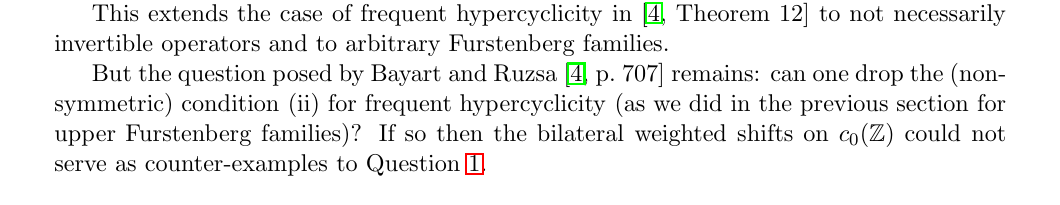
\includegraphics[width=\textwidth]{figures/later_open_status.png}
  \caption{The surviving non-symmetric condition in arXiv:1707.03994,
  PDF page 13.}
\end{figure}

We use the following invertible specialization of that characterization.
For every null sequence $\varepsilon_p>0$, frequent hypercyclicity of $B_w$
provides pairwise disjoint sets $E_p\subset\N$ with $\ud(E_p)>0$ such that
\begin{align}
 |n-m|&>p+q
 &&(n\in E_p,\ m\in E_q,\ n\ne m),                                   \tag{2}\\
 W_n&\longrightarrow\infty
 &&(n\to\infty,\ n\in E_p),                                          \tag{3}
\end{align}
and, writing $r=|n-m|$,
\[
       W_r>\frac1{\min(\varepsilon_p,\varepsilon_q)},
       \qquad
       L_r<\min(\varepsilon_p,\varepsilon_q).                          \tag{4}
\]
The published condition states one inequality for each ordering of $n,m$;
swapping the ordered pair gives the symmetric formulation (4).

The inverse is conjugate to the backward shift with
$w'_n=1/w_{-n+1}$.  Its cumulative products are
\[
                  W'_r=L_r^{-1},\qquad L'_r=W_r^{-1}.                   \tag{5}
\]
Thus (2) and (4) are already invariant under inversion.  Only the individual
condition (3) is missing on the inverse side.

\section{An unconditional positive-density escape theorem}

We first record a density diagonalization lemma.

\begin{lemma}[lower-density diagonal]\label{lem:diagonal}
Let $S_1\supset S_2\supset\cdots$ be subsets of $\N$ and suppose
$\ud(S_j)\geq\delta>0$ for every $j$.  There is $A\subset\N$ with
$\ud(A)\geq\delta$ such that $A\setminus S_j$ is finite for every $j$.
\end{lemma}

\begin{proof}
Choose increasing integers $N_j$ so that, whenever $N\geq N_j$,
\[
 \frac{|S_j\cap[0,N]|}{N+1}\geq\delta-\frac1j.
\]
Let $q(n)$ be a nondecreasing integer-valued function tending to infinity
such that $N_{q(n)}\leq n$ (define it arbitrarily before $N_1$), and set
\[
                         A=\{n:n\in S_{q(n)}\}.
\]
For $n\leq N$, one has $q(n)\leq q(N)$ and hence
$S_{q(N)}\subset S_{q(n)}$.  Therefore
\[
 |A\cap[0,N]|\geq|S_{q(N)}\cap[0,N]|
 \geq\left(\delta-\frac1{q(N)}\right)(N+1).
\]
This proves the density bound.  Once $q(n)\geq j$, membership in $A$ implies
membership in $S_{q(n)}\subset S_j$, proving the almost-containment.
\end{proof}

\begin{theorem}[simultaneous two-sided escape]\label{thm:escape}
If $B_w$ is invertible and frequently hypercyclic on $c_0(\Z)$, then there is
$\delta>0$ such that, for every $R\geq1$,
\[
 \ud\{r\geq1: W_r>R\ \text{and}\ L_r<R^{-1}\}\geq\delta.             \tag{6}
\]
Consequently there is a set $A\subset\N$ with $\ud(A)\geq\delta$ such that
\[
             W_r\longrightarrow\infty,\qquad L_r\longrightarrow0
             \quad(r\to\infty,\ r\in A).                             \tag{7}
\]
\end{theorem}

\begin{proof}
Take a witness family satisfying (2)--(4), and put $\delta=\ud(E_1)>0$.
Given $R$, choose $q$ so large that
$\min(\varepsilon_1,\varepsilon_q)<R^{-1}$, and fix $t\in E_q$.  If
$n\in E_1$ and $n>t$, then applying (4) to $n,t$ gives
\[
                    W_{n-t}>R,\qquad L_{n-t}<R^{-1}.
\]
The positive part of the translate $E_1-t$ has lower density $\delta$, which
proves (6).  Apply Lemma~\ref{lem:diagonal} to the decreasing sets
\[
                    S_j=\{r:W_r>j,\ L_r<1/j\}
\]
to obtain (7).
\end{proof}

This rules out the most direct counterexample strategy: the inverse cannot
fail merely because its positive cumulative products lack a positive-density
escape sequence.  What is not controlled is the product behavior on all
\emph{pairwise differences} of a full family of return-time sets.

\section{A tail-rich criterion that gives the full inverse conclusion}

Call a witness family $(E_p)$ in (2)--(4) \emph{tail-rich} if there exists
$A\subset\bigcup_pE_p$ with $\ud(A)>0$ such that
\[
 \ell(n)\longrightarrow\infty\quad(n\to\infty,\ n\in A),              \tag{8}
\]
where $\ell(n)=p$ for $n\in E_p$.  The label is well-defined because the
$E_p$ are disjoint.

\begin{theorem}[tail-rich inversion]\label{thm:tailrich}
If an invertible frequently hypercyclic bilateral shift $B_w$ admits a
tail-rich witness family, then $B_w^{-1}$ is frequently hypercyclic.
\end{theorem}

\begin{proof}
Fix $s$ and $t\in E_s$, and set
\[
                         B=(A-t)\cap\N.
\]
Then $\ud(B)=\ud(A)>0$.  Partition $B$ into sets $B_j$ of positive lower
density: if $B=\{b_0<b_1<\cdots\}$, one may assign $b_k$ to $B_j$ when
the $2$-adic valuation of $k+1$ is $j-1$.  Indeed,
\[
 |B_j\cap[0,N]|=2^{-j}|B\cap[0,N]|+O(1).                               \tag{9}
\]

Let $\eta_j=2^{-j}$.  Since $\varepsilon_p\to0$, choose $P_j\geq j$ such
that $\varepsilon_p\leq\eta_j$ for $p\geq P_j$.  By (8), deleting finitely
many points from each $B_j$ gives sets $F_j$ of positive lower density such
that
\[
             x+t\in E_p,\ x\in F_j\quad\Longrightarrow\quad p\geq P_j.
                                                                            \tag{10}
\]
For distinct $x\in F_j$ and $y\in F_k$, write
$x+t\in E_p$ and $y+t\in E_q$.  Translation preserves differences, so
(2), (4), and (10) give
\begin{align*}
 |x-y|&>p+q\geq j+k,\\
 L_{|x-y|}&<\min(\eta_j,\eta_k),\\
 W_{|x-y|}&>1/\min(\eta_j,\eta_k).
\end{align*}
By (5), these are exactly the separation and pairwise-product conditions for
$B_w^{-1}$.

It remains to check the individual non-symmetric condition.  If $x\in F_j$
and $x+t\in E_p$, then (4), applied to $x+t$ and the fixed point $t\in E_s$,
gives
\[
             L_x<\min(\varepsilon_p,\varepsilon_s)\leq\varepsilon_p.
\]
As $x\to\infty$ in $F_j$, (8) gives $p\to\infty$, hence $L_x\to0$ and
$W'_x=L_x^{-1}\to\infty$.  Grosse-Erdmann's characterization applied to
$(F_j)$ and $(\eta_j)$ proves that $B_w^{-1}$ is frequently hypercyclic.
\end{proof}

The hypothesis has a convenient sufficient form.

\begin{corollary}[tail-union test]\label{cor:tailunion}
For a witness family put $U_P=\bigcup_{p\geq P}E_p$.  If
\[
                         \inf_{P\geq1}\ud(U_P)>0,                       \tag{11}
\]
then $B_w^{-1}$ is frequently hypercyclic.
\end{corollary}

\begin{proof}
Apply Lemma~\ref{lem:diagonal} to the decreasing sets $U_P$.  The resulting
positive-density set is almost contained in every $U_P$, so its label tends
to infinity.  Theorem~\ref{thm:tailrich} applies.
\end{proof}

\begin{corollary}[monotone negative side]
If $L_r$ is eventually nonincreasing (in particular, if $w_n\leq1$ for all
sufficiently negative $n$), then $B_w^{-1}$ is frequently hypercyclic.
\end{corollary}

\begin{proof}
Theorem~\ref{thm:escape} and eventual monotonicity imply $L_r\to0$ on all of
$\N$.  Hence the original sets $E_p$ satisfy the missing individual condition
$W'_n=L_n^{-1}\to\infty$; (2), (4), and (5) provide every other condition.
\end{proof}

\section{Remaining obstruction}

Condition (11) is not automatic for a countable disjoint family of
positive-lower-density sets: their densities may decrease so fast that the
tail unions have lower density tending to zero.  Theorem~\ref{thm:escape}
does give uniformly dense product sublevel sets, but they contain different
common translates of the witness family.  Splicing those translates destroys
the pairwise-difference control in (4), replacing a controlled difference by
a four-term expression.  Conversely, a hierarchical counterexample must
respect (6)--(7), so merely making the negative products small on successively
sparser levels cannot work.

Eight focused routes were audited: exact literature status, symmetric product
reformulation, uniform-density extraction, density diagonalization, direct use
of one escape set, common-translation gluing, tail-union forcing, and a
hierarchical counterexample design.  The successful deductions are
Theorems~\ref{thm:escape} and \ref{thm:tailrich}; the unrestricted gluing step
remains open.

\begin{thebibliography}{9}
\bibitem{BR}
F. Bayart and I. Z. Ruzsa,
\emph{Difference sets and frequently hypercyclic weighted shifts},
Ergodic Theory Dynam. Systems 35 (2015), 691--709; arXiv:1305.2325.

\bibitem{GE}
K.-G. Grosse-Erdmann,
\emph{Frequently hypercyclic bilateral shifts},
Glasgow Math. J. 61 (2019), 271--286; arXiv:1707.03994.

\bibitem{Menet}
Q. Menet,
\emph{Inverse of frequently hypercyclic operators},
J. Inst. Math. Jussieu 21 (2022), 1867--1876; arXiv:1910.04452.
\end{thebibliography}

\end{document}
